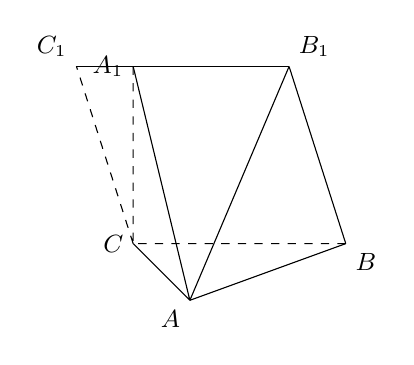
\begin{tikzpicture}[x=0.9cm,y=0.9cm,every node/.style={font=\small}]
  \coordinate (A)  at (1.8,0.2);
  \coordinate (B)  at (4,1);
  \coordinate (C)  at (1,1);
  \coordinate (A1) at (1,3.5);
  \coordinate (B1) at (3.2,3.5);
  \coordinate (C1) at (0.2,3.5);

  % 棱柱可见棱、遮挡棱，以及原图中标出的 A_1C 与 AB_1
  \draw (A)--(B) (A)--(C) (A)--(A1);
  \draw (A1)--(B1) (B1)--(C1) (C1)--(A1);
  \draw (B)--(B1) (A)--(B1);
  \draw[dashed] (B)--(C) (C)--(C1) (A1)--(C);

  \node[below left] at (A) {$A$};
  \node[below right] at (B) {$B$};
  \node[left] at (C) {$C$};
  \node[left] at (A1) {$A_1$};
  \node[above right] at (B1) {$B_1$};
  \node[above left] at (C1) {$C_1$};
\end{tikzpicture}
